\documentclass[12pt,a4paper]{article}
\usepackage[margin=1.25in]{geometry}
\usepackage{fancyhdr} % fancy header
\pagestyle{fancy} % so fancy
\usepackage[russian,english]{babel} % for russian letters
\usepackage{tipa} % for IPA symbols
\usepackage[round]{natbib} % bibliography
\usepackage{graphicx} % for importing graphics / figures
\usepackage{booktabs} % publication-worthy tables
\usepackage{adjustbox} % makes tables fit nicely on the page
\usepackage{hyperref}


\lhead{Josh Meyer}
\rhead{DeepSpeech WIP}
\cfoot{} %% make empty to get rid of the page number %% \cfoot{Page \thepage}
\renewcommand{\footrulewidth}{0.4pt} %% this puts a fancy line at the footer


\begin{document}

\subsection*{UTF-8}

Branch: \href{https://github.com/mozilla/DeepSpeech/tree/utf8}{\texttt{utf8}}

UTF-8 training on 100 hours // Jobs on cluster: 4640, 4637, 4641, 4642

\begin{center}
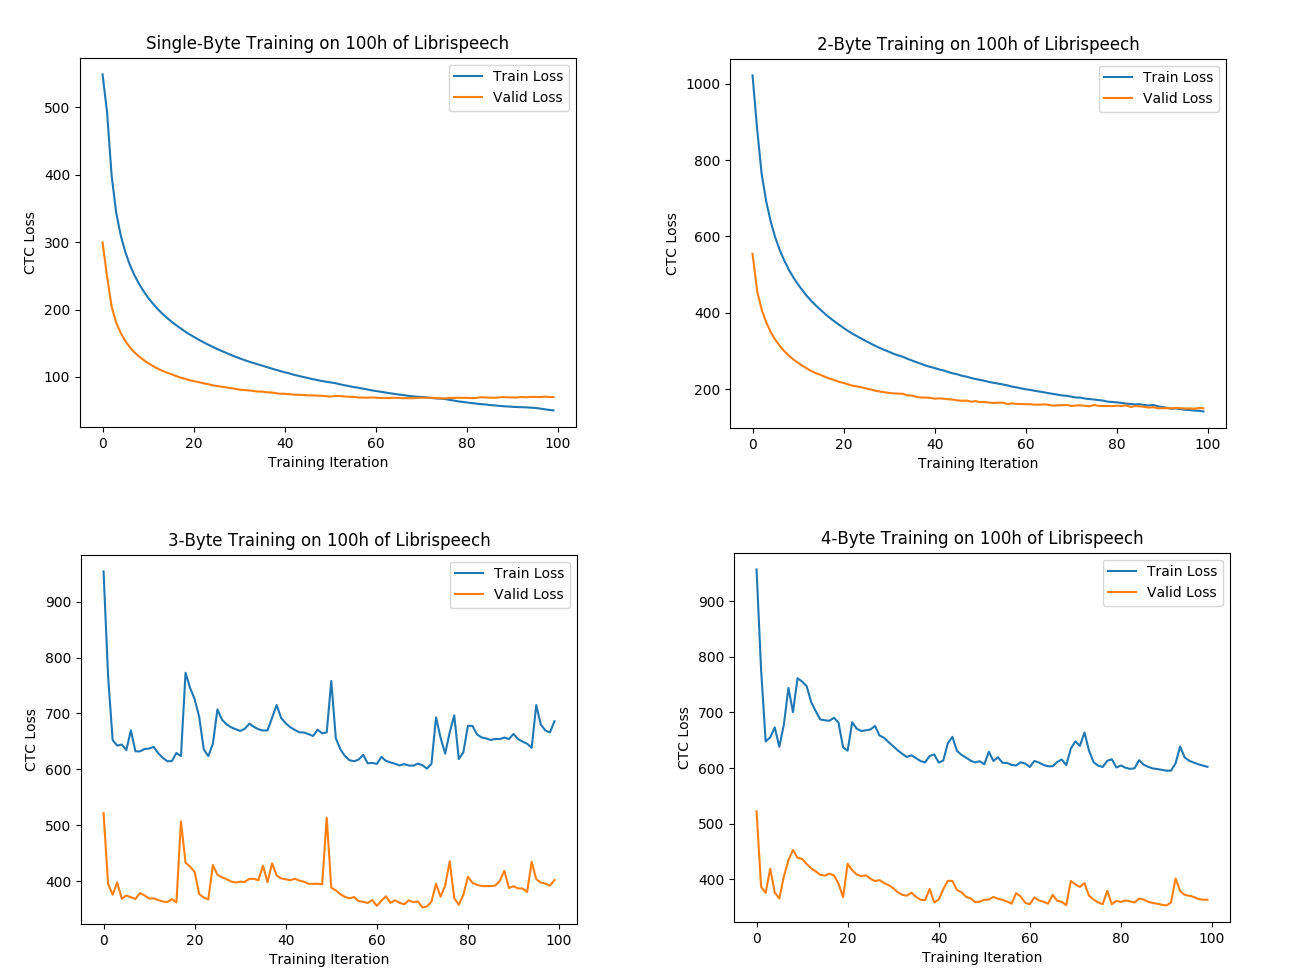
\includegraphics[width=.85\textwidth,keepaspectratio]{figs/3.png}
\end{center}

UTF-8 training on 3,000 hours // Jobs on cluster: 4650, 4651, 4652, 4653

\begin{center}
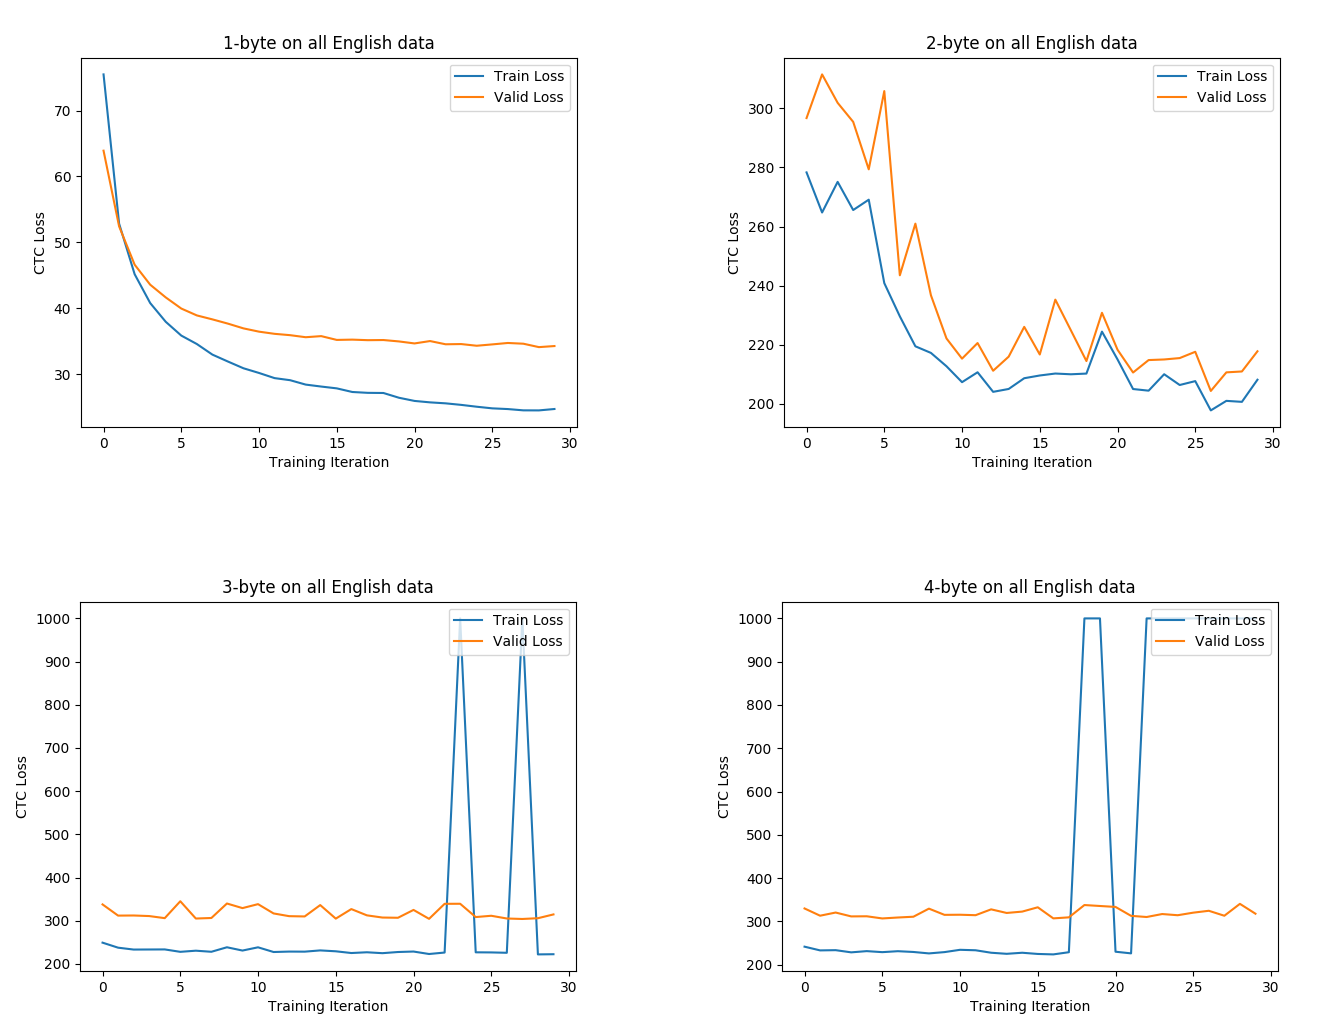
\includegraphics[width=.85\textwidth,keepaspectratio]{figs/4.png}
\end{center}


\subsubsection*{UTF-8 Decoding + different Language Models}
The following are decoding results from the English training on LibriSpeech, Switchboard, and Fisher. The \textbf{new} language model was compiled exactly as specified in the \texttt{lm/data} \href{https://github.com/mozilla/DeepSpeech/tree/master/data/lm}{\texttt{README}}, including the same dataset from OpenSLR.

The \textbf{old} language model was a bi-gram built on Wikipedia (if I recall correctly).

\begin{center}
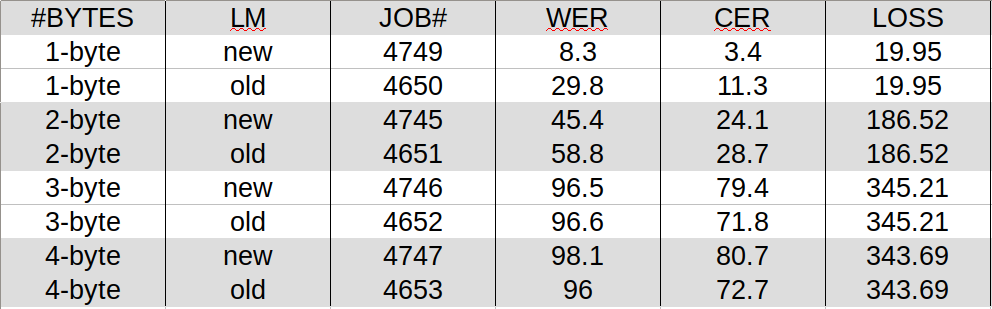
\includegraphics[width=.85\textwidth,keepaspectratio]{figs/1.png}
\end{center}




\subsection*{Transfer Learning}

Branch: \href{https://github.com/mozilla/DeepSpeech/tree/transfer-learning}{\texttt{transfer-learning}}
Branch: \href{https://github.com/mozilla/DeepSpeech/tree/transfer-learning2}{\texttt{transfer-learning2}}

The \texttt{transfer-learning} branch should be replaced by \texttt{transfer-learning2} once we can verify the former is working correctly. The former is based on a more current master.

These branches both assume the output layer is at the character level, not the byte level.


\subsection*{UTF8 + Transfer Learning}

Branch: \href{https://github.com/mozilla/DeepSpeech/tree/transfer-utf8}{\texttt{transfer-utf8}}

Jobs on Cluster: 4752

This branch assumes decoding at the byte level, but is agnostic as to whether or not the source model was trained on bytes or characters.
\newpage

\subsection*{UTF-8 + more LSTMs}

Branch: \href{https://github.com/mozilla/DeepSpeech/tree/nLSTMS-utf8}{\texttt{nLSTMS-utf8}}

Job on cluster: 4753 (in queue to train on 3,000 hours of English with 2 LSTMs)

UTF-8 training on Single Sentence:

\begin{center}
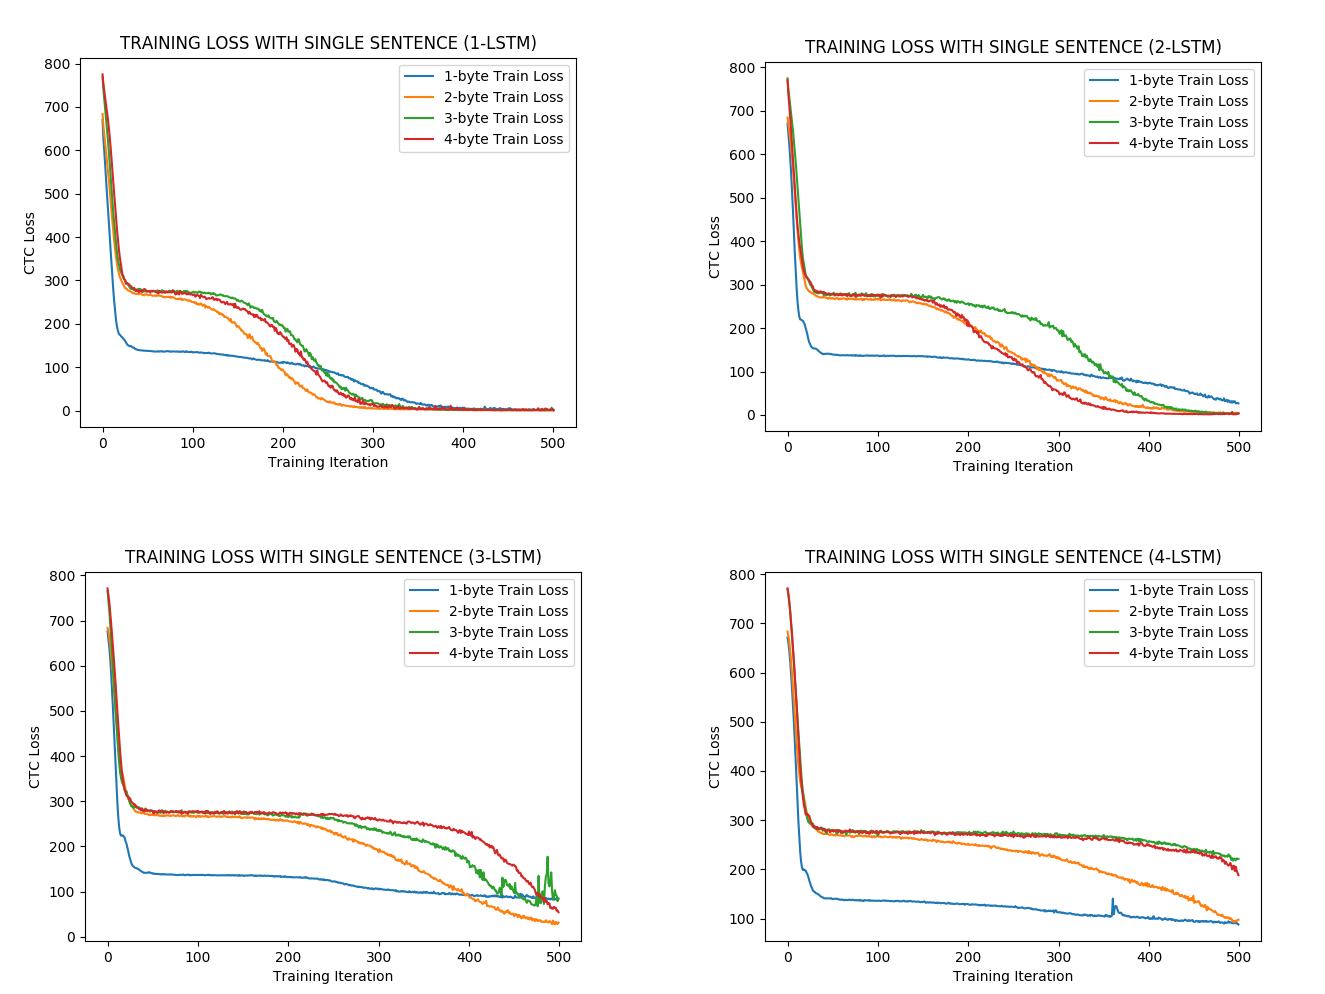
\includegraphics[width=.85\textwidth,keepaspectratio]{figs/2.png}
\end{center}

\subsection*{Miscellaneous}

I made a lot of branches that were language specific, and they can be deleted. These language-specific branches were a hack around having LM data on the server. Specifically, all the \texttt{transfer-learning-*} branches may be deleted, as well at the \texttt{utf8-*} branches.


\end{document}

